\section{Multiplexor 4 a 1 \label{sec:s2}}

\begin{center}
	\begin{minipage}{12cm}
		\begin{tcolorbox}[title=Actividad 2]
			Completar el código del multiplexor 4 a 1 en el lenguaje de su elección primero usando estructura \textit{'case'} y después \textit{'ifs'} anidados. Compilar y simular. Usar el visor RTL para establecer si hay diferencias en el resultado de la síntesis de los dos casos. implementar en la tarjeta DE2-115 solo el caso de la estructura \textit{''case''}.
		\end{tcolorbox}	
	\end{minipage}
\end{center}

La visualización RTL del multiplexor 4 a 1 en Verilog se muestra en la \autoref{fig:mux_4_1_case_rtl} utilizando la estructura \textit{case} y en la \autoref{fig:mux_4_1_if_rtl} utilizando la estructura \textit{if}. Como se observa, el multiplexor con la estructura \textit{case} se implementa empleando una instancia de multiplexor 4 a 1, con un tamaño de selección de 2 bits, en cambio, el que se describió con estructura \textit{if} hace uso de varios elementos lógicos, específicamente 4 comparadores de magnitud y 4 multiplexores 2 a 1. Las simulaciones para el código en Verilog se visualizan en la \autoref{fig:mux_4_1_case_WaveBi} para el multiplexor de estructura \textit{case} y en la \autoref{fig:mux_4_1_if_WaveBi} para el de la estructura \textit{if}. Los bits de entrada fueron escogidos de tal forma que se observe de manera clara el funcionamiento del módulo.

En los Anexos se localiza la descripción de las dos implementaciones de multiplexor. Para el primer caso se utilizó la sentencia \textit{case} para evaluar cada estado de la variable de control SEL, todo esto dentro de una lista sensible. En cambio, para el segundo caso se usó una sentencia \textit{if} por cada estado de la variable SEL, igualmente dentro de una lista sensible.

\begin{figure}[ht]
	\centering
	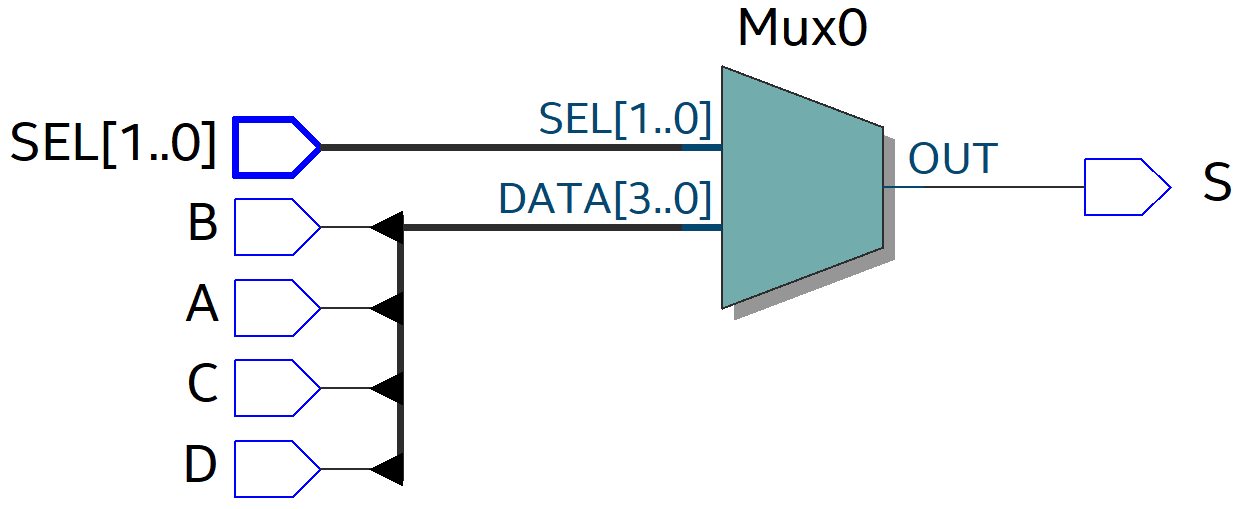
\includegraphics[scale=0.4]{Mux_4_1_Case_RTL.png}
	\caption{Diagrama RTL del multiplexor 4 a 1, utilizando la estructura \textit{case}. \label{fig:mux_4_1_case_rtl}}
\end{figure}

\begin{figure}[ht]
	\centering
	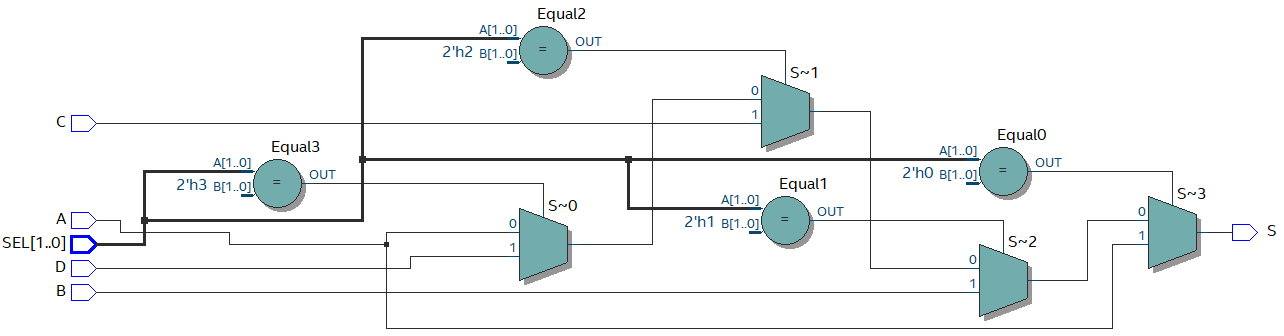
\includegraphics[scale=0.5]{Mux_4_1_If_RTL.png}
	\caption{Diagrama RTL del multiplexor 4 a 1, utilizando la estructura \textit{if}. \label{fig:mux_4_1_if_rtl}}
\end{figure}

\begin{figure}[ht]
	\centering
	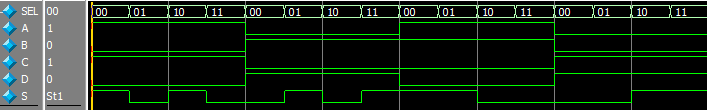
\includegraphics[scale=0.9]{Mux_4_1_Case_WaveBi.png}
	\caption{Simulación del multiplexor 4 a 1, utilizando la estructura \textit{case} con el visor de formas de onda de ModelSim. 
	\label{fig:mux_4_1_case_WaveBi}}
\end{figure}

\begin{figure}[ht]
	\centering
	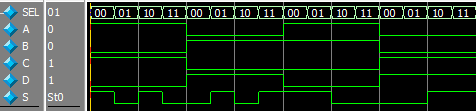
\includegraphics[scale=1.3
	 ]{Mux_4_1_If_WaveBi.png}
	\caption{Simulación del multiplexor 4 a 1, utilizando la estructura \textit{if} con el visor de formas de onda de ModelSim. 
	\label{fig:mux_4_1_if_WaveBi}}
\end{figure}





